\documentclass{standalone}
\usepackage{tikz}
\usepackage{amsmath}

\begin{document}
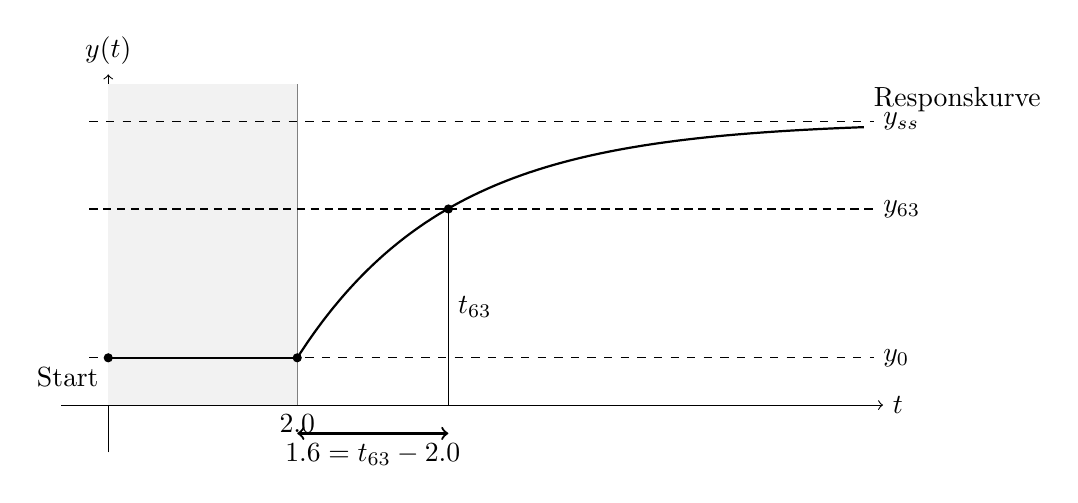
\begin{tikzpicture}[scale=1.2]

% --- Parameters ---
\def\y0{0.5}
\def\yss{3.0}
\def\theta{2.0}
\def\tau{1.6}

% Precomputed 63% level:
% y63 = y0 + 0.63*(yss-y0) = 0.5 + 0.63*2.5 = 2.075
\def\ySixtyThree{2.075}

% Precomputed t63 = theta + tau
\def\tSixtyThree{3.6}

% --- Axes ---
\draw[->] (-0.5,0) -- (8.2,0) node[right] {$t$};
\draw[->] (0,-0.5) -- (0,3.5) node[above] {$y(t)$};

% --- Dead time shading ---
\fill[gray!10] (0,0) rectangle (\theta,3.4);
\draw[gray] (\theta,0) -- (\theta,3.4);
\node[below] at (\theta,0) {$\theta$};

% --- Response curve (simple exponential shape) ---
\draw[domain=\theta:8, smooth, samples=200, thick]
      plot (\x, {\yss - (\yss-\y0)*exp(-(\x-\theta)/\tau)});

% Before dead time
\draw[thick] (0,\y0) -- (\theta,\y0);

% --- Reference lines ---
\draw[dashed] (-0.2,\y0) -- (8.1,\y0) node[right] {$y_0$};
\draw[dashed] (-0.2,\yss) -- (8.1,\yss) node[right] {$y_{ss}$};

% 63% level
\draw[dash pattern=on 3pt off 2pt]
      (-0.2,\ySixtyThree) -- (8.1,\ySixtyThree)
      node[right] {$y_{63}$};

% Vertical line at t63
\draw[thin] (\tSixtyThree,0) -- (\tSixtyThree,\ySixtyThree)
      node[midway,right] {$t_{63}$};

% Arrow showing tau
\draw[<->, thick] (\theta,-0.3) -- (\tSixtyThree,-0.3)
      node[midway,below] {$\tau = t_{63}-\theta$};

% Point markers
\filldraw (0,\y0) circle (1.2pt);
\filldraw (\theta,\y0) circle (1.2pt);
\filldraw (\tSixtyThree,\ySixtyThree) circle (1.2pt);

% Labels
\node[below left] at (0,\y0) {Start};
\node[above right] at (8, {3.0}) {Responskurve};

\end{tikzpicture}
\end{document}